\section{Langkah-Langkah Percobaan}
Pada percobaan pertama yaitu crimping dan pengaturan routing IPv4, kami mengawali proses dengan menyiapkan perlengkapan seperti kabel UTP, konektor RJ45, tang crimping, serta LAN tester. Kabel UTP kami susun mengikuti pola warna standar T568B untuk menjamin kualitas koneksi. Setelah penyusunan selesai, konektor RJ45 dipasangkan ke ujung kabel menggunakan tang crimping. 
Untuk mengecek keberhasilan proses ini, kabel diuji menggunakan LAN tester guna memastikan semua jalur koneksi bekerja sebagaimana mestinya. 

Saat melakukan konfigurasi routing IPv4 dengan aplikasi Winbox, langkah awal yang kami lakukan adalah mereset kedua router ke pengaturan default agar tidak terjadi konflik pada pengaturan sebelumnya. Kami membuka Winbox dan masuk ke masing-masing router menggunakan MAC address atau IP default, dengan username "admin" dan tanpa password jika belum ditentukan sebelumnya. Setelah berhasil login, konfigurasi dimulai dengan menetapkan IP address pada interface ether1 yang difungsikan sebagai jalur antar router. Router pertama dikonfigurasi dengan IP 10.10.10.1/30, dan router kedua dengan IP 10.10.10.2/30.

Selanjutnya, kami melanjutkan konfigurasi pada interface ether2 untuk koneksi ke jaringan lokal. IP address yang diberikan pada router pertama adalah 192.168.10.1/27, sedangkan pada router kedua adalah 192.168.20.1/27.
Untuk mengarahkan lalu lintas antar jaringan, kami menambahkan routing statis pada kedua router. Di menu IP -> Routes, kami menetapkan rute pada router pertama menuju jaringan 192.168.20.0/27 melalui gateway 10.10.10.2, dan pada router kedua menuju jaringan 192.168.10.0/27 melalui gateway 10.10.10.1.

Langkah berikutnya adalah memberikan konfigurasi IP secara manual pada perangkat laptop yang terhubung ke masing-masing router. Laptop pada router pertama diberi IP 192.168.10.2 dengan gateway 192.168.10.1, sementara laptop pada router kedua diberi IP 192.168.20.2 dengan gateway 192.168.20.1.
Sebagai bentuk pengujian akhir, kami melakukan ping dari laptop yang terhubung ke router pertama ke laptop pada router kedua. Jika proses ping berhasil tanpa kendala, maka dapat disimpulkan bahwa konfigurasi routing IPv4 berhasil dilakukan dan perangkat dalam jaringan mampu saling terhubung.

\section{Analisis Hasil Percobaan}
Dalam pelaksanaan percobaan Crimping, kami berhasil melakukan proses penyambungan kabel menggunakan peralatan yang telah disediakan. Namun, pada kabel LAN pertama, kami menghadapi kendala karena urutan warna kabel tidak mengikuti standar yang ditetapkan. Akibatnya, koneksi tidak dapat terbentuk dengan baik. Untuk mengatasinya, kami memotong ulang kabel tersebut dan menyusun kembali urutan warnanya sesuai standar yang benar. Setelah dilakukan perbaikan dan crimping ulang, kabel dapat terpasang dengan tepat dan koneksi berhasil terjalin dengan lancar.

Sementara itu, dalam percobaan Routing IPv4, kami menemui beberapa kesulitan dalam melakukan konfigurasi IP statis. Walaupun telah mengikuti langkah-langkah yang seharusnya, percobaan tidak dapat diselesaikan hingga waktu yang tersedia habis. Permasalahan utama berasal dari kesalahan konfigurasi alamat IP, khususnya pada laptop kedua yang tersambung ke router kedua. Perangkat tersebut memiliki alamat IP default dari Google yang tidak dapat dihapus, sehingga proses komunikasi menjadi terganggu dan koneksi antar perangkat gagal tercapai. Akibatnya, konfigurasi routing statis pun tidak berhasil diterapkan sepenuhnya.

Kami juga sempat mencoba melanjutkan dengan konfigurasi routing IPv4 dinamis. Namun, keterbatasan waktu membuat kami tidak sempat menyelesaikan proses tersebut. Rencana untuk menerapkan routing dinamis menggunakan protokol RIP pun terpaksa tertunda karena pengaturan belum sempat dilakukan.



\section{Hasil Tugas Modul}
Pada simulasi jaringan menggunakan Cisco Packet Tracer, saya merancang sebuah topologi jaringan yang terdiri dari dua router, dua switch, dan delapan perangkat PC yang terbagi menjadi empat departemen, dengan masing-masing dua PC per departemen. Setiap router dikonfigurasi dengan menambahkan modul NM-4E untuk menyediakan port Ethernet tambahan. Port-port tersebut digunakan untuk menghubungkan router dengan switch, serta antar-router melalui jaringan backbone. Konfigurasi dilakukan dengan menetapkan alamat IP yang sesuai pada setiap interface, baik di sisi router maupun PC, sesuai subnet yang telah dirancang. Routing statis kemudian diterapkan agar komunikasi antar jaringan lokal (LAN) dapat berlangsung. Setiap PC dikonfigurasi secara manual melalui menu Desktop > IP Configuration untuk menetapkan IP address, subnet mask, dan default gateway. Setelah konfigurasi selesai, pengujian konektivitas dilakukan dengan perintah ping antar PC lintas jaringan untuk memastikan routing berjalan dengan baik. Simulasi ini bertujuan untuk memahami implementasi dasar jaringan komputer, termasuk crimping virtual, segmentasi jaringan, konfigurasi IP, serta penerapan routing statis antar router.


\subsection{Struktur Jaringan}
\begin{figure}[H]
  \centering
  \begin{minipage}[t]{0.48\textwidth}
    \centering
    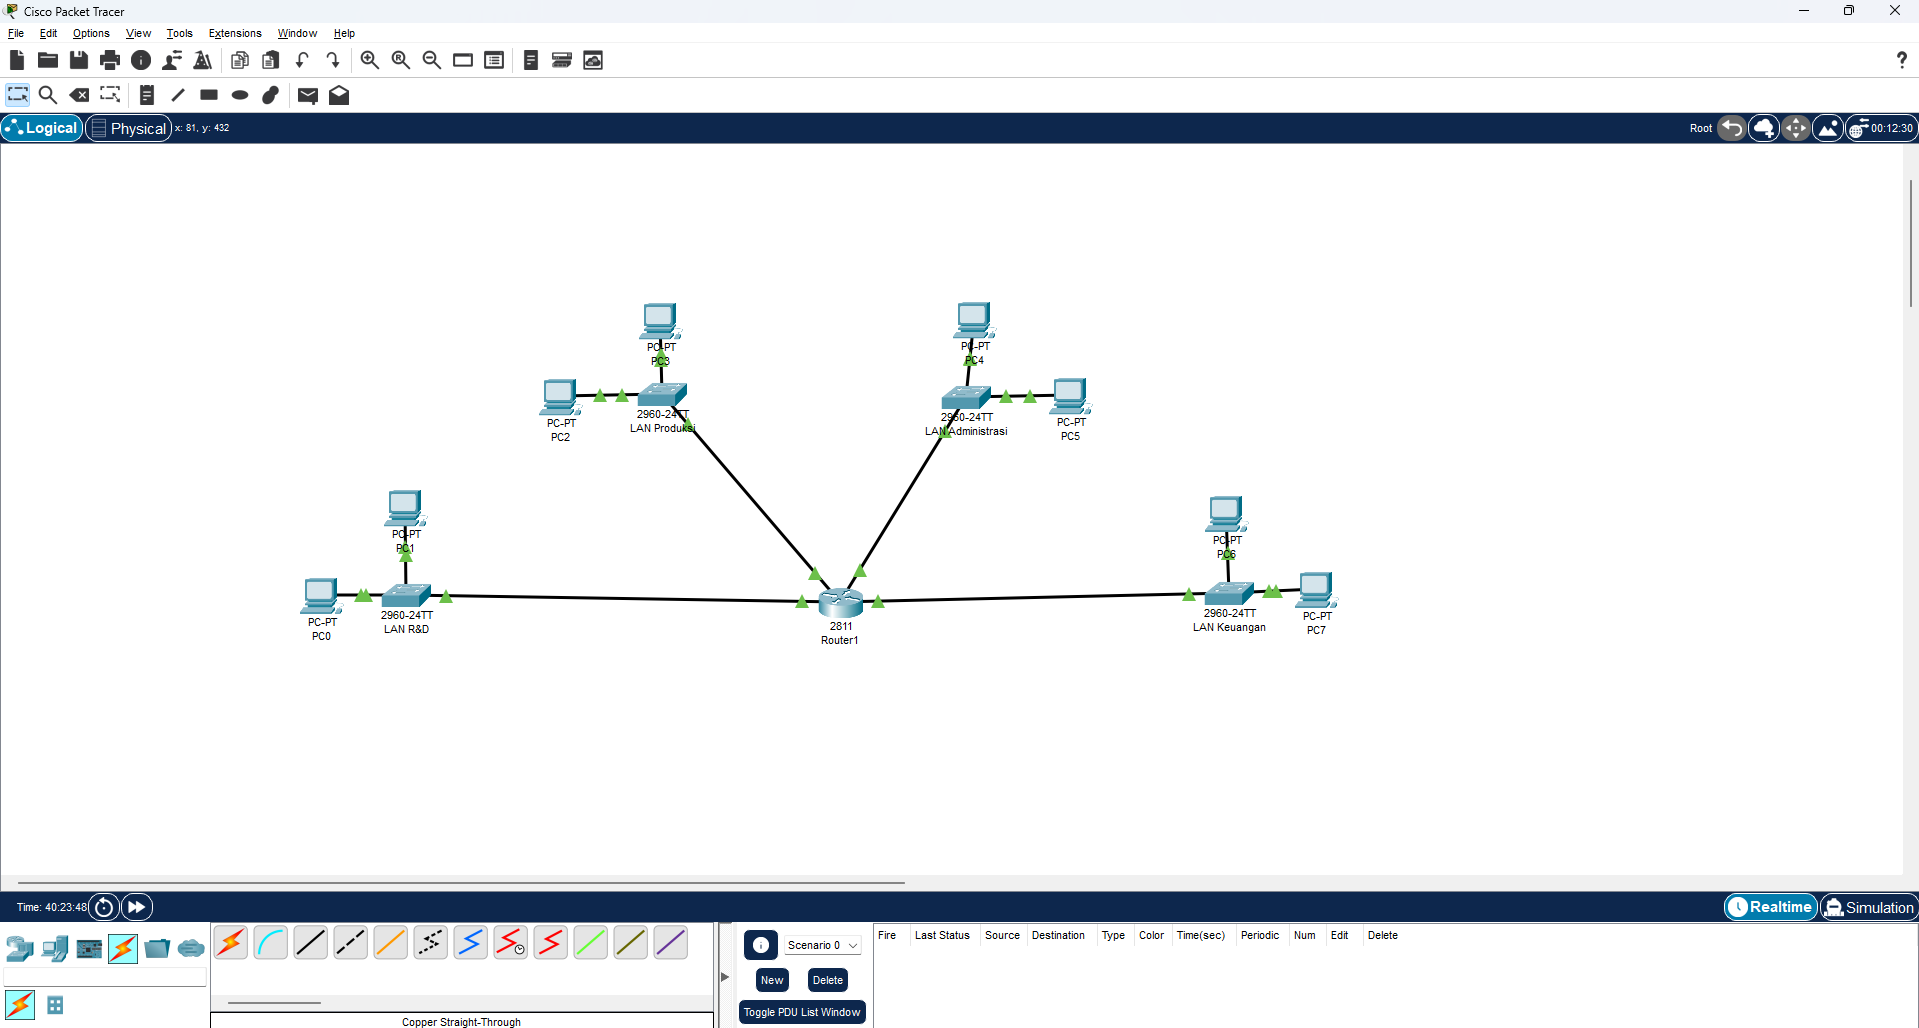
\includegraphics[width=\linewidth]{P1/img/StrukturJaringan.png}
    \caption{Struktur Jaringan Keseluruhan}
    \label{fig:struktur}
  \end{minipage}
  \hfill
  \begin{minipage}[t]{0.48\textwidth}
    \centering
    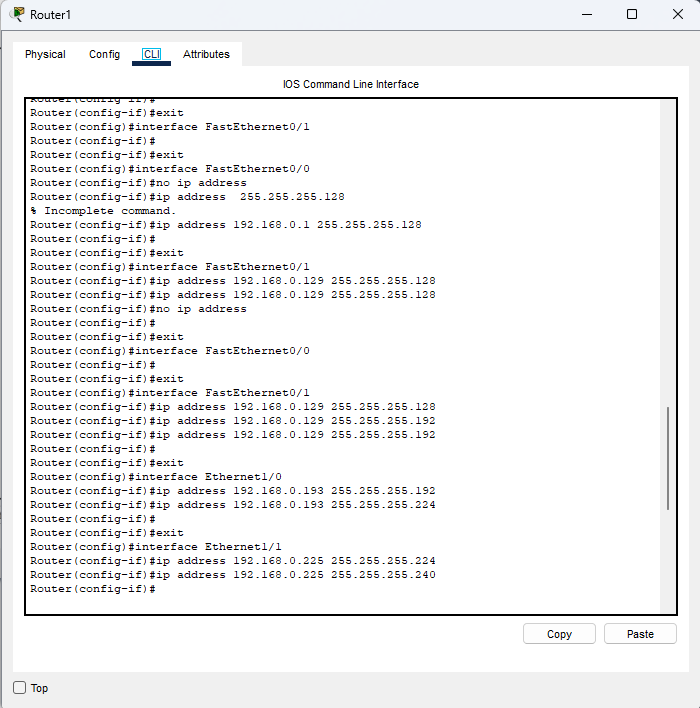
\includegraphics[width=\linewidth]{P1/img/cli.png}
    \caption{CLI Router Utama}
    \label{fig:cli}
  \end{minipage}
\end{figure}

\begin{figure}[H]
  \centering
  \begin{minipage}[t]{0.48\textwidth}
    \centering
    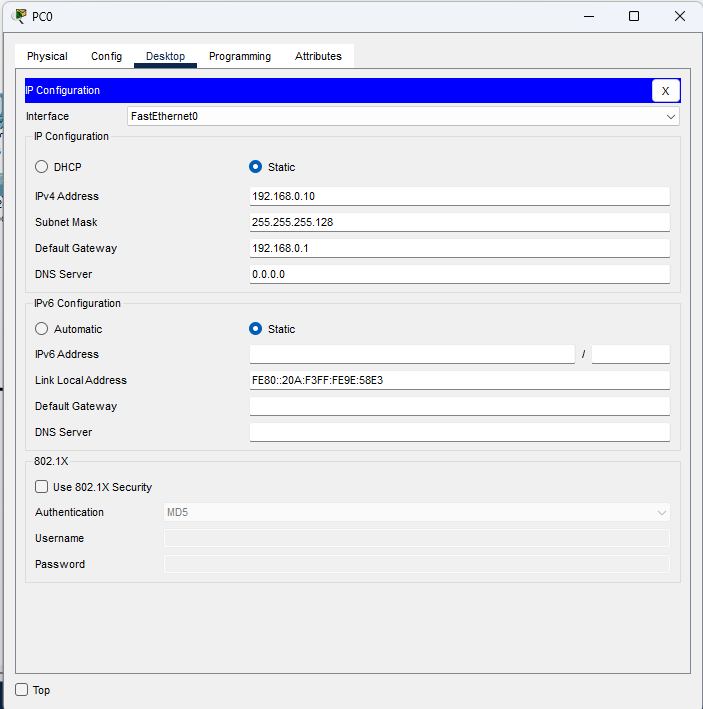
\includegraphics[width=\linewidth]{P1/img/IPr&D.png}
    \caption{Address R\&D}
    \label{fig:rnd}
  \end{minipage}
  \hfill
  \begin{minipage}[t]{0.48\textwidth}
    \centering
    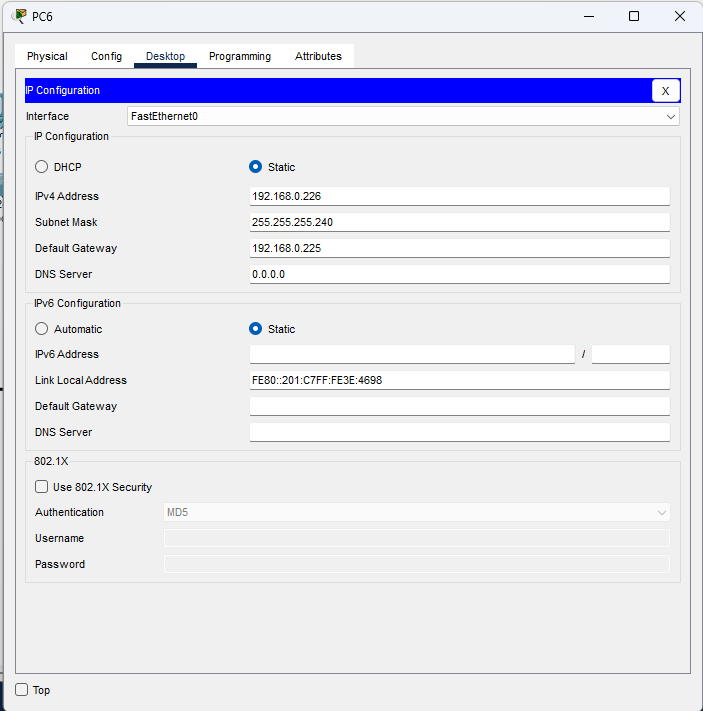
\includegraphics[width=\linewidth]{P1/img/IPkeu.png}
    \caption{Address Finance}
    \label{fig:finance}
  \end{minipage}
\end{figure}

\begin{figure}[H]
  \centering
  \begin{minipage}[t]{0.48\textwidth}
    \centering
    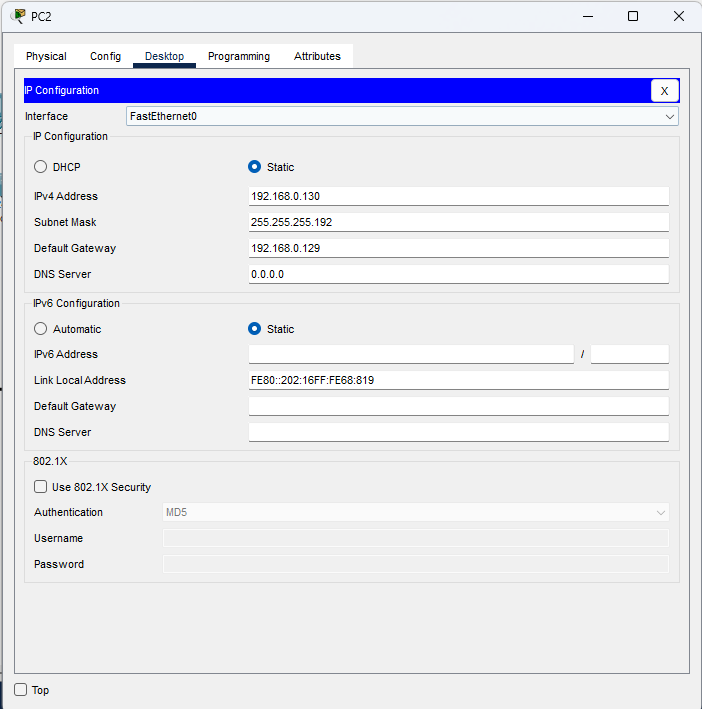
\includegraphics[width=\linewidth]{P1/img/IPprod.png}
    \caption{Address Production}
    \label{fig:production}
  \end{minipage}
  \hfill
  \begin{minipage}[t]{0.48\textwidth}
    \centering
    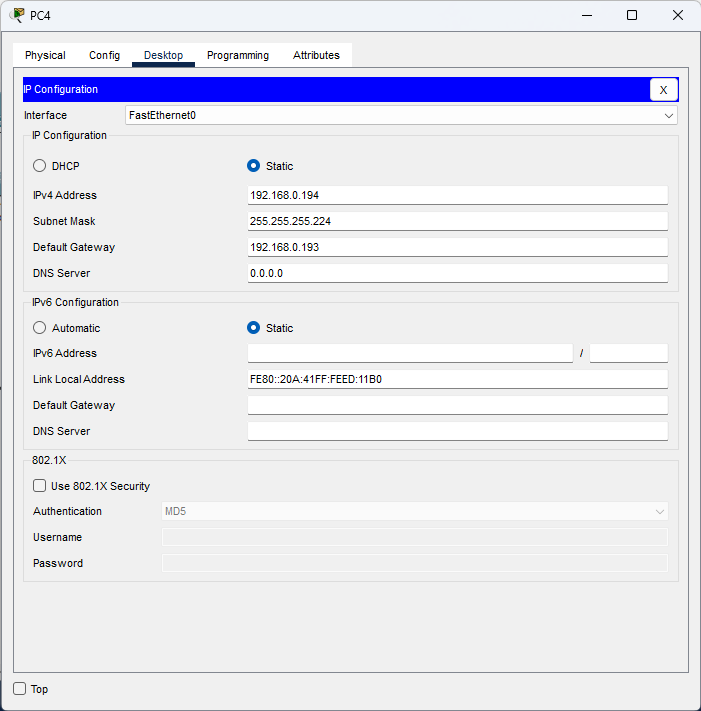
\includegraphics[width=\linewidth]{P1/img/IPadm.png}
    \caption{Address Administration}
    \label{fig:admin}
  \end{minipage}
\end{figure}

\section{Kesimpulan}
Berdasarkan percobaan yang telah dilakukan, dapat disimpulkan bahwa proses crimping kabel memerlukan ketelitian tinggi, terutama dalam menyusun urutan warna kabel sesuai standar. Meskipun sempat mengalami kendala pada kabel pertama, setelah dilakukan perbaikan, koneksi dapat terjalin dengan baik, menandakan keberhasilan proses crimping. Sementara itu, pada percobaan routing IPv4, kendala teknis dalam pengaturan alamat IP—khususnya adanya IP bawaan yang tidak dapat dihapus—menghambat proses konfigurasi statis dan mengakibatkan gagalnya komunikasi antar jaringan. Keterbatasan waktu juga menjadi faktor utama yang menyebabkan konfigurasi routing dinamis tidak sempat diselesaikan. Hal ini menunjukkan pentingnya manajemen waktu dan pemahaman yang lebih mendalam terhadap konfigurasi IP dan routing dalam praktik jaringan.

\section{Lampiran}
\subsection{Dokumentasi saat praktikum}
\begin{figure}[H]
    \centering
    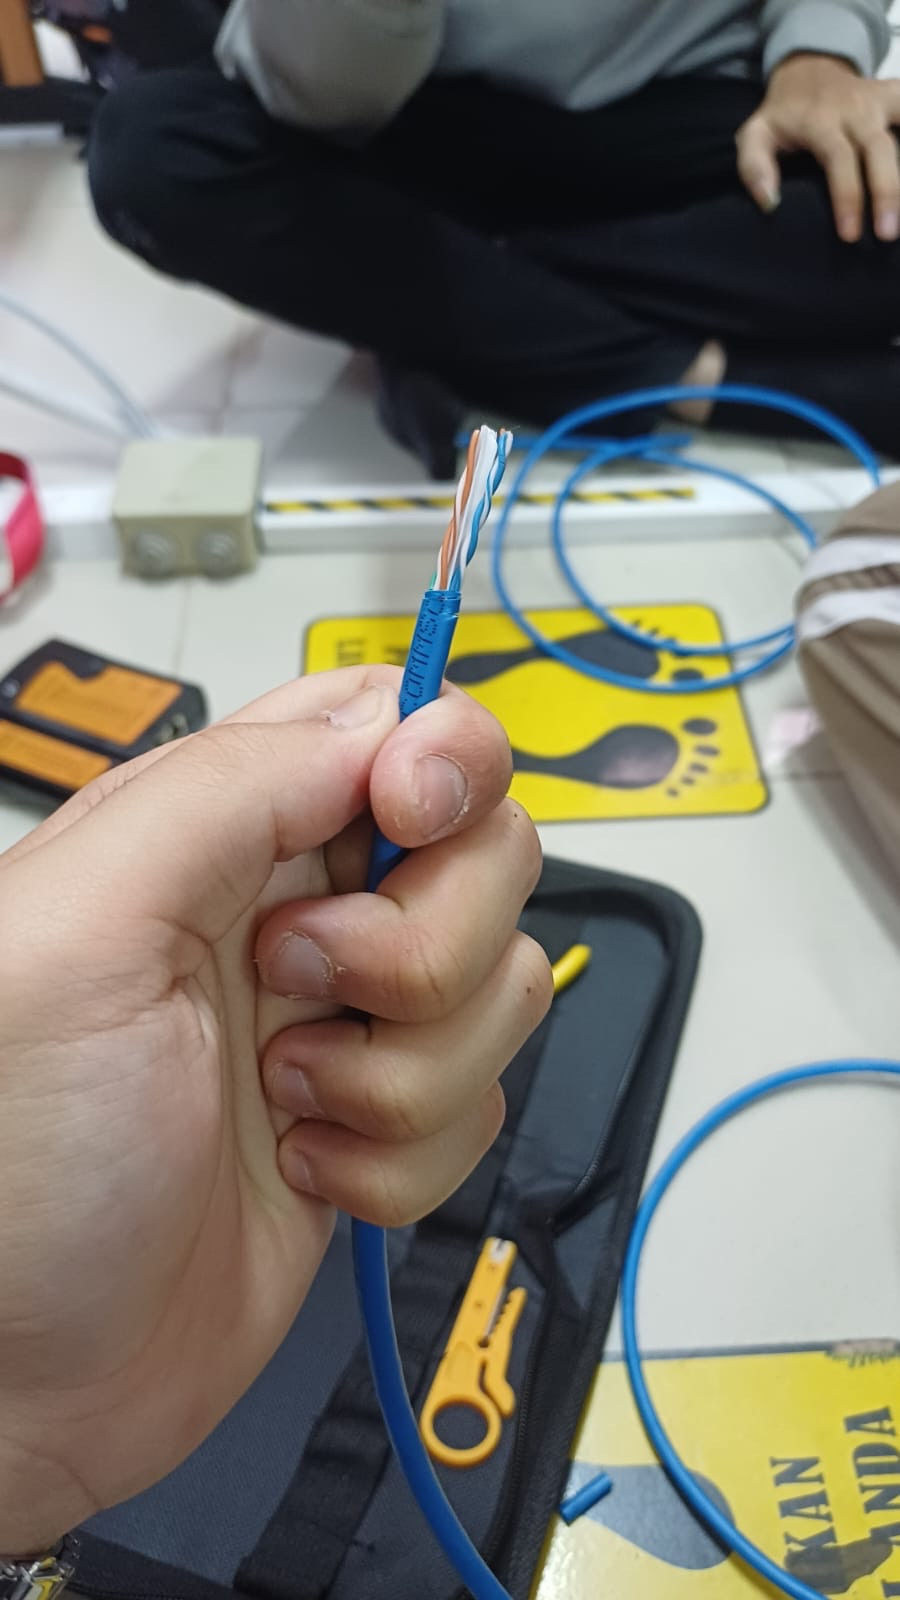
\includegraphics[width=0.48\textwidth]{P1/img/kabelsebelumcrimping.jpg}
    \caption{Kabel sudah tersusun sebelum crimping}
    \label{fig:crimping2_lampiran}
\end{figure}

\newpage
Pengujian kabel hasil crimping dengan LAN Tester untuk memastikan bahwa setiap kabel terhubung dengan benar

\begin{figure}[H]
    \centering
    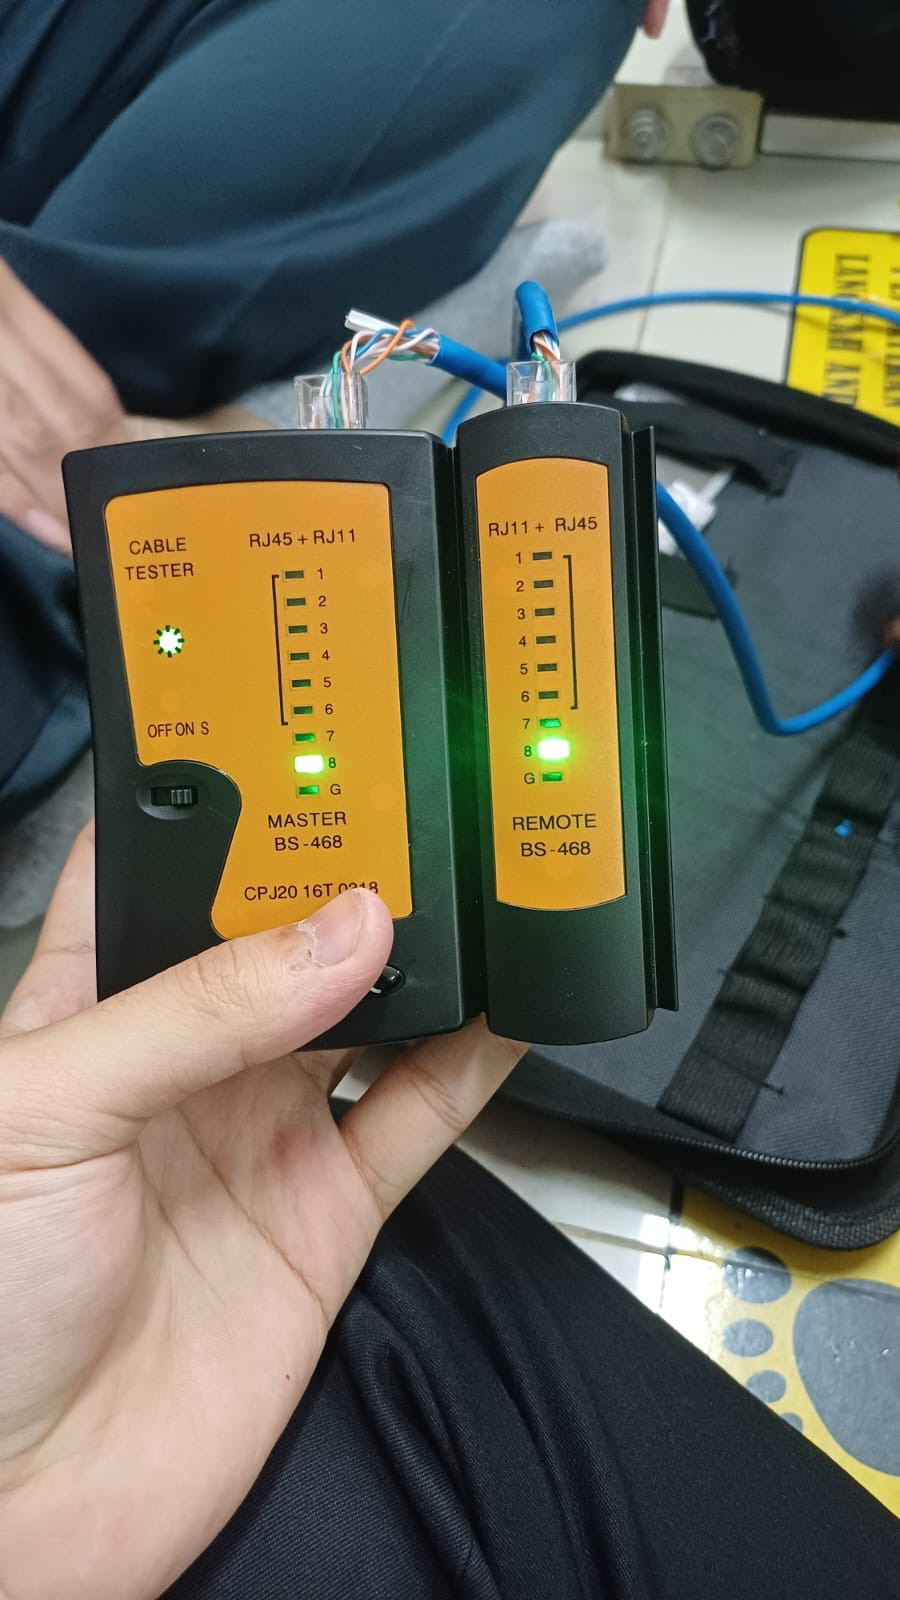
\includegraphics[width=0.48\textwidth]{P1/img/lantester.jpg}
    \caption{Kabel sudah tersusun sebelum crimping}
    \label{fig:crimping2_lampiran}
\end{figure}

Kabel hasil crimping yang telah selesai

\begin{figure}[H]
    \centering
    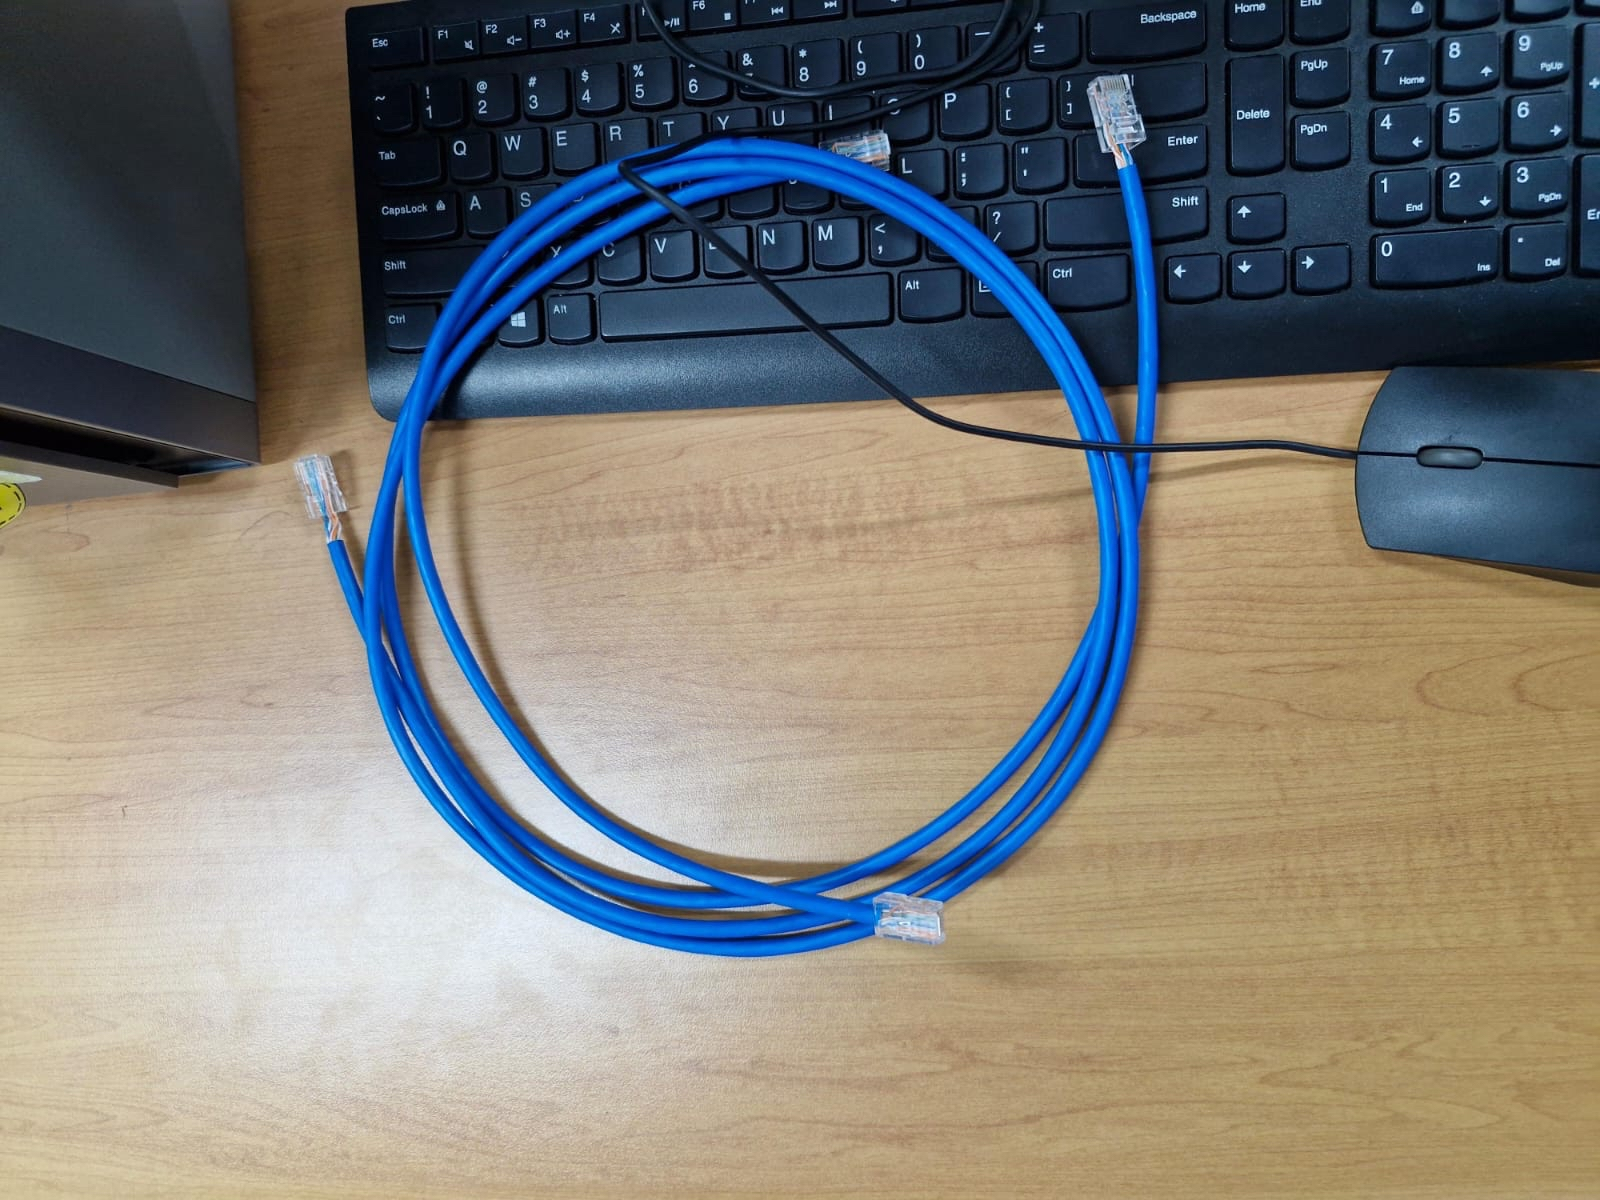
\includegraphics[width=0.48\textwidth]{P1/img/hasilcrimping.jpg}
    \caption{Kabel sudah tersusun sebelum crimping}
    \label{fig:crimping2_lampiran}
\end{figure}
